\documentclass[11pt]{article}

\usepackage[letterpaper, margin=1in]{geometry}
\usepackage{graphicx}
\usepackage{booktabs}
\usepackage{amsmath}
\usepackage{amssymb}
\usepackage{caption}
\usepackage{subcaption}
\usepackage{hyperref}
\usepackage{url}
\usepackage{xcolor}
\usepackage{microtype}

\hypersetup{
  colorlinks=true,
  linkcolor=blue!60!black,
  urlcolor=blue!60!black,
  citecolor=blue!60!black
}

\graphicspath{{../results/figures/}}

\title{Real-Data Driven Denoising Autoencoders for 1D Periodic Time-Series Signals}
\author{Nikhil Pesaladinne \and Islam Tayeb \\ CS 675 --- Project 2}
\date{April 2026}

\begin{document}
\maketitle

\begin{abstract}
This project implements a denoising autoencoder pipeline for 1D periodic time-series signals, with the synthetic training benchmark grounded in statistics measured from a real dataset. We extract weekly Wikipedia pageviews for five articles with strong annual seasonality, fit a dominant-sinusoid model to each, and characterize the resulting residual distribution. Three candidate noise models (Gaussian, masking, impulse) are then fit to those residuals; the best-fitting one by Wasserstein distance (Gaussian) is combined with the fitted sine distribution to generate a labelled synthetic training corpus. Two architectures (MLP, 1D CNN) are compared. The CNN denoiser achieves $+15.2$\,dB SNR improvement on the synthetic test set with roughly half the parameter count of the MLP, a clean latent-dimension knee at 16, and graceful generalization to noise intensities up to $3\times$ its training level. A per-article sine-recovery test evaluates the trained CNN under conditions that match its training assumptions: each article's fitted sine is corrupted by the fitted Gaussian noise and run through the autoencoder. The CNN delivers $+8.9$ to $+11.9$\,dB SNR improvement against the known sine and passes clean sines through at $\sim$65\,dB SNR. As an extension, the same model is applied via overlap-averaged sliding windows to the raw Wikipedia series themselves; the reconstruction improves SNR against the fitted-sine proxy by $+2.3$ to $+8.1$\,dB. The smaller gain on the raw series reflects that the windowed reconstruction also captures non-stationary structure (year-to-year amplitude variation, phase drift) that a single global sine cannot represent.
\end{abstract}

\section{Introduction}

A denoising autoencoder learns a mapping $f_\theta: x_{\text{noisy}} \mapsto \hat{x}$ that recovers a clean signal $x$ from a corrupted observation $x_{\text{noisy}} = x + \varepsilon$, by minimizing a reconstruction loss $\mathcal{L}(\theta) = \mathbb{E}\,\| x - f_\theta(x_{\text{noisy}}) \|_2^2$. For 1D signals this is a well-established setup. This project implements the pipeline end-to-end while grounding the synthetic training distribution in statistics measured from a real dataset, so the trained model can be evaluated both on synthetic data with true ground truth and on the real series it was ultimately intended for.

The pipeline has six stages:
\begin{enumerate}
  \item Pull weekly Wikipedia pageviews for five articles with known annual cycles (\texttt{Influenza, Common\_cold, Fever, Cough, Christmas}).
  \item Fit a dominant-sinusoid model and treat it as a \emph{proxy} clean signal.
  \item Compute residuals (real $-$ fit), characterize their statistics, and select one of three candidate noise models by goodness-of-fit.
  \item Sample from the distribution of fitted sines and corrupt with the selected noise model to produce labelled synthetic training pairs.
  \item Train and compare two denoising autoencoder architectures (MLP, 1D CNN) on the synthetic data.
  \item Evaluate the trained CNN on synthetic test data, on a per-article sine-recovery task that matches the training assumptions, and as an extension on the raw real Wikipedia series.
\end{enumerate}
This report documents the dataset, architectures, and quantitative results from each stage, along with the visualizations used in the evaluation.

\section{Dataset}\label{sec:data}

\paragraph{Source.} Daily English-Wikipedia pageviews for five articles --- four disease/symptom articles with a known winter-peaked annual cycle (\texttt{Influenza}, \texttt{Common\_cold}, \texttt{Fever}, \texttt{Cough}) and one positive-control article (\texttt{Christmas}) --- pulled from the public Wikimedia Pageviews REST API \cite{wikimedia} for the span 2018-01-01 through the present. Each daily series is resampled to weekly totals (Monday-anchored) and aligned across articles, yielding five concurrent series of length $T = 472$ weeks.

\paragraph{Transform.} All downstream processing operates on $y = \log(1 + \text{pageviews})$. The log transform stabilizes variance (raw pageviews span more than two orders of magnitude across articles) and makes the dominant annual cycle approximately sinusoidal in the transformed domain, which is the assumption every later step depends on.

\paragraph{Why these articles.} The disease articles all have well-documented annual cycles tied to the Northern-Hemisphere flu season, which gives the project a real signal to denoise. \texttt{Christmas} is included as a positive control: its annual cycle is essentially deterministic and large-amplitude, so any pipeline that fails on \texttt{Christmas} is broken. We do not claim Wikipedia pageviews are a clean reflection of disease incidence; we only claim they have enough structure to test denoising machinery against.

\section{Method}

\subsection{Sine-wave fitting (proxy clean signal)}\label{sec:sinefit}
For each article's log-pageview series $y[t]$ of length $T$, we fit
\begin{equation}
\hat{y}[t] = c + m\,t + A\,\sin\!\bigl(2\pi f\, t + \varphi\bigr),
\end{equation}
by initializing the dominant frequency from a Hanning-windowed FFT, then refining $(c, m, A, f, \varphi)$ jointly with bounded least squares. The frequency search is restricted to $\pm 50\%$ of the FFT estimate. Per-article goodness of fit $R^2$ is reported in Section~\ref{sec:results-fit}.

\subsection{Residual characterization}
Residuals $r[t] = y[t] - \hat{y}[t]$ are pooled across articles and characterized by mean, standard deviation, skewness, excess kurtosis, fraction of $|r| > 3\sigma$ outliers, fraction of near-zero values ($|r| < 0.05\sigma$), lag-1 autocorrelation, and the longest run with $|r| < 0.1\sigma$. These statistics inform both the noise-model selection and the interpretation of the final results.

\subsection{Noise models}\label{sec:noise}
Three noise models are implemented per the project specification:
\begin{itemize}
  \item \textbf{Gaussian.} $x_{\text{noisy}} = x + \varepsilon$, $\varepsilon \sim \mathcal{N}(0, \sigma^2)$. One parameter $\sigma$.
  \item \textbf{Masking.} For each window, draw $n \sim \mathrm{Pois}(\lambda_{\text{rate}})$ segments of length $\ell \sim \mathrm{Pois}(\bar{\ell})$ and replace the values in each segment with the local window mean. Two parameters $(\lambda_{\text{rate}}, \bar{\ell})$.
  \item \textbf{Impulse.} Each index has independent probability $p$ of receiving an additive spike; spike magnitude is $\pm \kappa\sigma_x \cdot (1 + 0.5\,\mathcal{N}(0,1))$ where $\sigma_x$ is the clean signal std. Two parameters $(p, \kappa)$.
\end{itemize}
Each model has a closed-form parameter estimator from the observed residuals (sample $\sigma$ for Gaussian; near-zero run statistics for masking; outlier rate and magnitude for impulse).

\subsection{Goodness-of-fit and noise selection}\label{sec:noiseselect}
Given the observed pooled residuals $r$ and a candidate noise model, we apply the model to the per-article fitted sines to produce synthetic residuals $\tilde{r}$, then score the match between $r$ and $\tilde{r}$ by:
\begin{itemize}
  \item Wasserstein distance (primary score, lower is better),
  \item Kolmogorov--Smirnov statistic and $p$-value,
  \item Excess-kurtosis and standard-deviation gaps,
  \item Difference in fraction-near-zero.
\end{itemize}
The best-fitting noise model (lowest Wasserstein) is used as the default for downstream architecture, latent, and noise-level experiments.

\subsection{Synthetic dataset generation}
From the fitted parameters $\{(c_i, m_i, A_i, f_i, \varphi_i)\}_{i=1}^5$ we construct a \texttt{SineFitDistribution} by taking the per-parameter min/max range with mild jitter (50\% on frequency to give the model variety, 25\% on amplitude/intercept). At dataset-build time each clean window of length $L = 128$ is rendered with parameters drawn uniformly from this distribution and then z-scored. The corresponding noisy window is produced by the selected noise model with the parameters fitted in Section~\ref{sec:noiseselect}. We generate 8000 train, 1000 validation, 1000 test windows per experiment.

\subsection{Architectures}\label{sec:arch}
Both architectures share the encoder--decoder interface $z = \mathrm{Enc}(x_{\text{noisy}})$, $\hat{x} = \mathrm{Dec}(z)$ with $\dim(z) < L$ and operate on input shape $(B, 1, L)$.
\begin{itemize}
  \item \textbf{MLPAE.} $L \to 256 \to 64 \to z \to 64 \to 256 \to L$, ReLU activations between dense layers.
  \item \textbf{CNN1DAE.} Encoder: \texttt{Conv1d} stack with kernel sizes $\{7,5,3\}$ and stride $2$ each, channel progression $1\to 16\to 32\to 64$, halving the temporal length three times, followed by a linear projection to $z$. Decoder mirrors with \texttt{ConvTranspose1d} (output\_padding chosen to recover length $L$ exactly) and a final $1\!\times\!1$ \texttt{Conv1d}.
\end{itemize}
The default latent dimension is $z = 16$ unless otherwise stated.

\subsection{Training and evaluation}
Loss is mean squared error between $\hat{x}$ and the true clean window. Optimizer: Adam, learning rate $10^{-3}$, batch size 64, up to 50 epochs with early stopping on validation loss (patience 10). Best weights are restored before test-set evaluation. Metrics:
\begin{align}
\mathrm{MSE}(x, \hat{x}) &= \tfrac{1}{NL}\sum_{n,t} (x_n[t] - \hat{x}_n[t])^2, \\
\mathrm{SNR}_{\mathrm{dB}}(x, \hat{x}) &= 10 \log_{10}\!\left(\frac{\|x\|_2^2}{\|x - \hat{x}\|_2^2}\right), \\
\Delta\mathrm{SNR} &= \mathrm{SNR}_{\mathrm{dB}}(x, \hat{x}) - \mathrm{SNR}_{\mathrm{dB}}(x, x_{\text{noisy}}).
\end{align}
SNR is averaged per-sample (clipped to $[-100, 100]$\,dB to handle the perfect-recon case).

\section{Experiments and Results}\label{sec:results}

\subsection{Sine fits and residuals (Exp 1)}\label{sec:results-fit}

\begin{table}[h]
\centering
\caption{Per-article sine fits in log-pageview space.}
\label{tab:sine_fits}
\begin{tabular}{lrrrrr}
\toprule
Article & $A$ & $f$ (cycles/wk) & period (wk) & $R^2$ & $\sigma_{\text{resid}}$ \\
\midrule
Influenza   & 0.380 & 0.0195 & 51.3  & 0.633 & 0.396 \\
Common\_cold & 0.307 & 0.0196 & 51.1  & 0.589 & 0.347 \\
Fever       & 0.136 & 0.0197 & 50.9  & 0.776 & 0.204 \\
Cough       & 0.186 & 0.0033 & 300.9 & 0.570 & 0.289 \\
Christmas   & 0.897 & 0.0192 & 52.1  & 0.554 & 0.566 \\
\bottomrule
\end{tabular}
\end{table}

Four of the five articles converge on the expected $\approx\!52$-week annual cycle. \texttt{Cough} is degenerate: the fit lands on a $\approx 6$-year period instead of the annual one, presumably because the article's annual amplitude is small relative to a long-term trend. We retain it as part of the dataset for honesty but flag this case in the discussion. Residual standard deviations are 0.14--0.57 in log-pageview units; excess kurtosis ranges from 3.6 (\texttt{Christmas}) to 38.0 (\texttt{Fever}), so all residual streams are heavier-tailed than Gaussian. Lag-1 autocorrelation is uniformly high (0.69--0.90), confirming the noise is far from i.i.d.\ and the fitted sine has missed real structure --- a fact we return to in Section~\ref{sec:discussion}.

\begin{figure}[h]
\centering
\begin{subfigure}{0.49\linewidth}
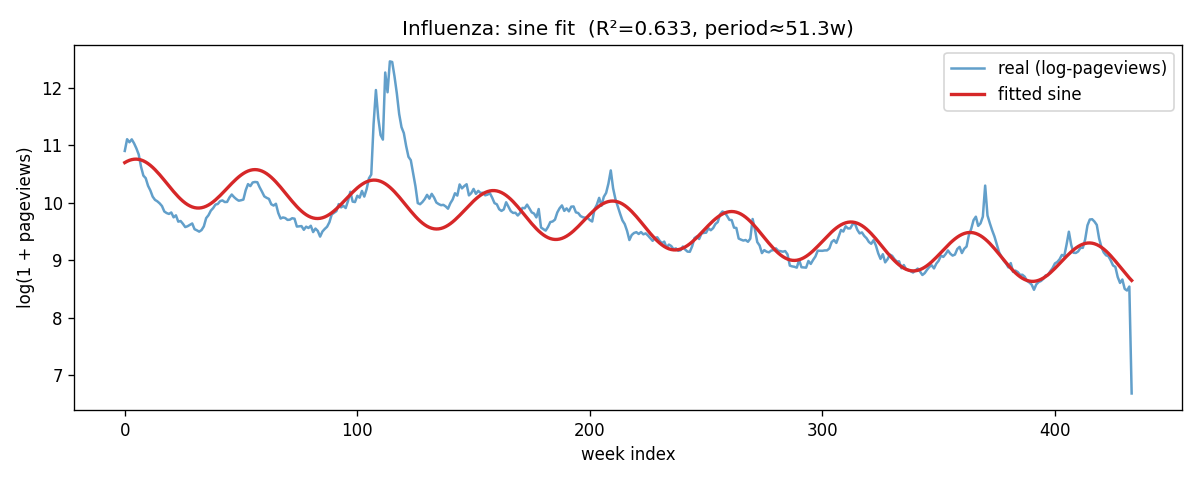
\includegraphics[width=\linewidth]{exp_1_fit/Influenza_sine_fit.png}
\caption{Influenza ($R^2 = 0.63$).}
\end{subfigure}
\hfill
\begin{subfigure}{0.49\linewidth}
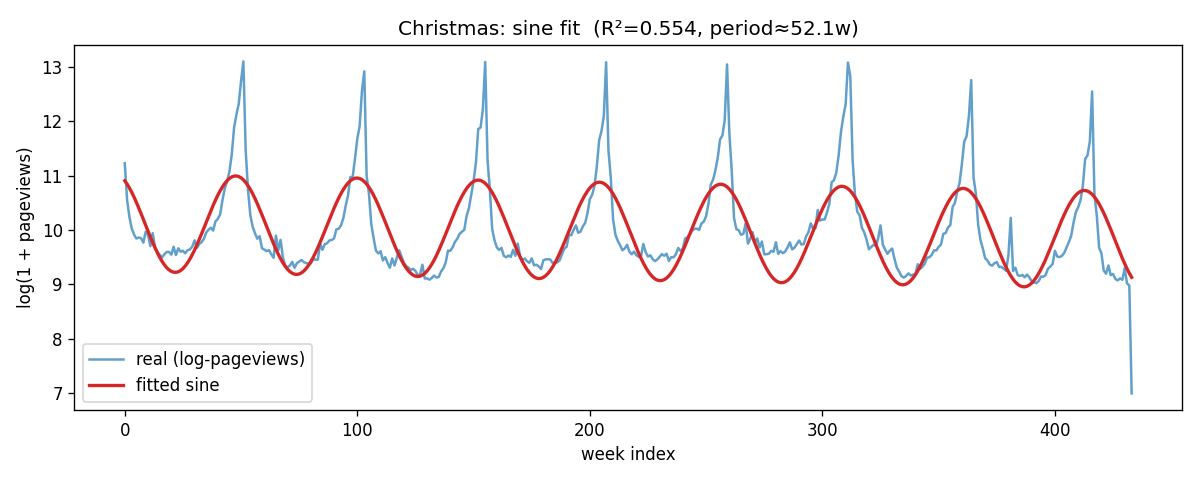
\includegraphics[width=\linewidth]{exp_1_fit/Christmas_sine_fit.png}
\caption{Christmas ($R^2 = 0.55$).}
\end{subfigure}
\caption{Real log-pageview series (blue) overlaid with the fitted sine (red). Both articles show clear annual cycles, but the fixed-amplitude global sine cannot track year-to-year amplitude variation.}
\label{fig:sine_fits}
\end{figure}

\subsection{Noise model selection (Exp 2)}\label{sec:results-noise}

\begin{table}[h]
\centering
\caption{Noise-model selection scores, ranked by Wasserstein distance to the pooled observed residuals.}
\label{tab:noise_select}
\begin{tabular}{lrrrrl}
\toprule
Kind & Wass.\ $\downarrow$ & KS stat & kurt.\ diff & $\sigma$ ratio & params \\
\midrule
\textbf{gaussian} & \textbf{0.106} & \textbf{0.118} & $-10.06$ & 0.999 & $\sigma = 0.380$ \\
masking          & 0.241 & 0.569 & $\phantom{-}819.5$  & 0.111 & $\lambda = 9.32,\ \bar{\ell} = 1.76$ \\
impulse          & 0.275 & 0.559 & $\phantom{-0}48.97$ & 1.908 & $p = 0.021,\ \kappa = 4.52$ \\
\bottomrule
\end{tabular}
\end{table}

Gaussian wins by a factor of $2.3\times$ on Wasserstein distance and matches the observed standard deviation almost exactly ($\sigma$-ratio $= 0.999$). Its weakness is the kurtosis gap ($-10.06$): the synthetic Gaussian cannot reproduce the heavy tails seen in the observed residuals. The two heavier-tailed candidates (masking and impulse) over-correct in the opposite direction --- impulse over-shoots $\sigma$ by $1.9\times$, masking under-shoots by an order of magnitude --- and both fail the bulk-distribution test (KS statistic $> 0.55$). All three candidates have effectively zero KS $p$-values; none is a perfect statistical match. We use Gaussian (the closest candidate) as the default for downstream experiments.

\begin{figure}[h]
\centering
\begin{subfigure}{0.49\linewidth}
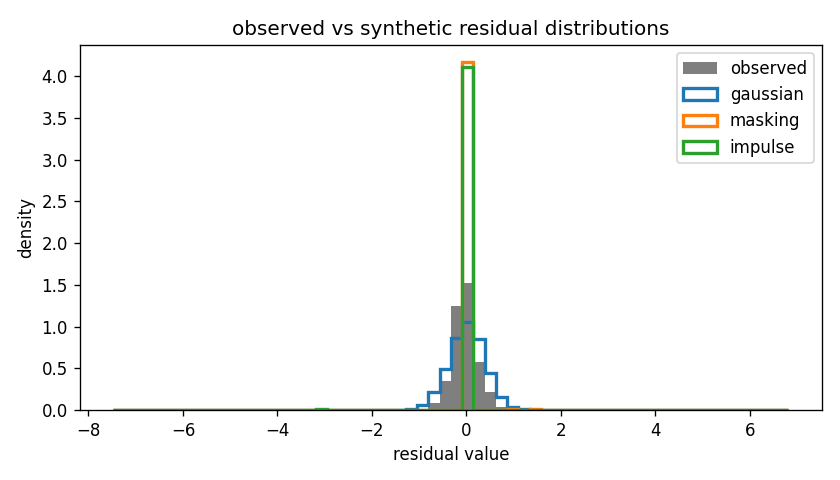
\includegraphics[width=\linewidth]{exp_2_noise_select/residual_hist_overlay.png}
\caption{Distribution overlay.}
\end{subfigure}
\hfill
\begin{subfigure}{0.49\linewidth}
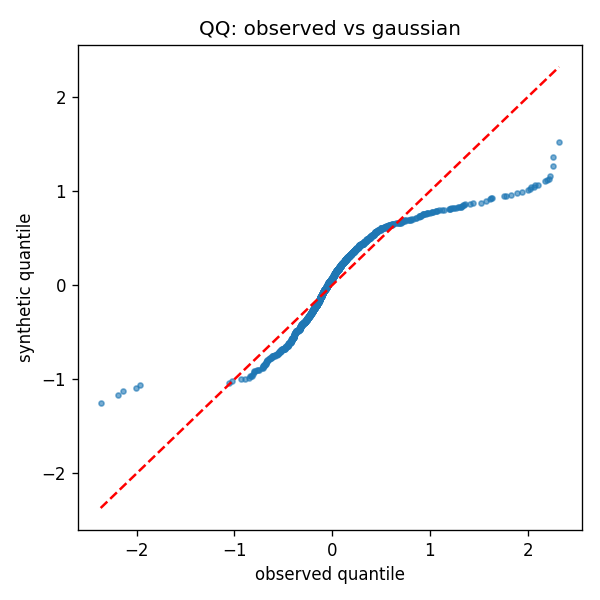
\includegraphics[width=\linewidth]{exp_2_noise_select/qq_gaussian.png}
\caption{Gaussian QQ plot vs.\ observed.}
\end{subfigure}
\caption{Noise-model selection. The Gaussian distribution matches the bulk of the residuals but cannot reproduce the heavy tails (visible as deviation from the diagonal at the QQ plot extremes).}
\label{fig:noise_select}
\end{figure}

\subsection{Architecture comparison (Exp 3)}

\begin{table}[h]
\centering
\caption{Architecture comparison on the synthetic test set with Gaussian noise at the fitted intensity.}
\label{tab:arch}
\begin{tabular}{lrrrrr}
\toprule
Model & Params & Test MSE $\downarrow$ & SNR$_{\text{out}}$ (dB) & $\Delta$SNR (dB) $\uparrow$ & Train (s) \\
\midrule
mlp   & 101\,136 & 0.00632 & 22.95 & 14.49 & \phantom{00}56.8 \\
\textbf{cnn1d} & \textbf{53\,313} & \textbf{0.00525} & \textbf{23.63} & \textbf{15.18} & 585.7 \\
\bottomrule
\end{tabular}
\end{table}

The 1D CNN achieves the best reconstruction error using only $\sim$53\% of the MLP's parameters. The MLP is competitive but consistently a few percent worse. We report the CNN as the canonical model used downstream.

\begin{figure}[h]
\centering
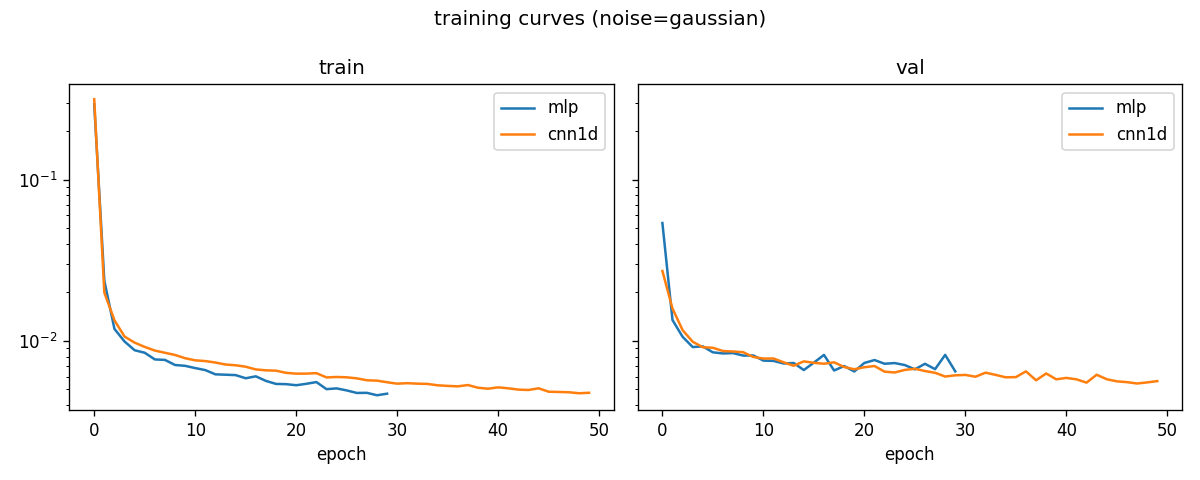
\includegraphics[width=0.85\linewidth]{exp_3_arch/training_curves.png}
\caption{Training and validation loss across architectures (log $y$-axis). Both models converge cleanly.}
\label{fig:training_curves}
\end{figure}

\begin{figure}[h]
\centering
\begin{subfigure}{0.49\linewidth}
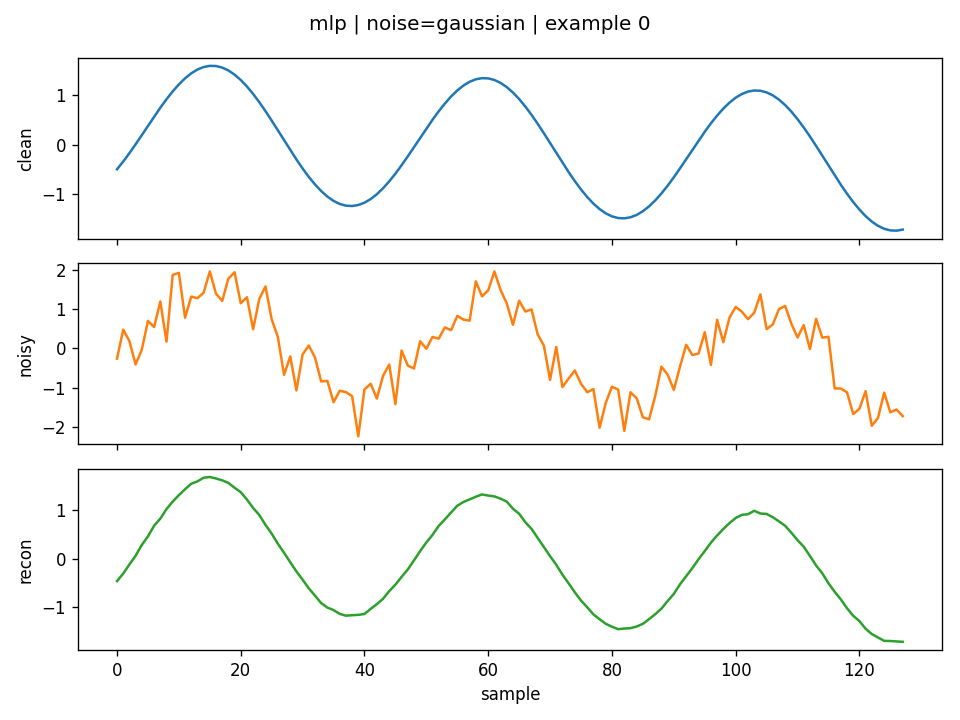
\includegraphics[width=\linewidth]{exp_3_arch/triplet_mlp_0.png}
\caption{MLP.}
\end{subfigure}
\hfill
\begin{subfigure}{0.49\linewidth}
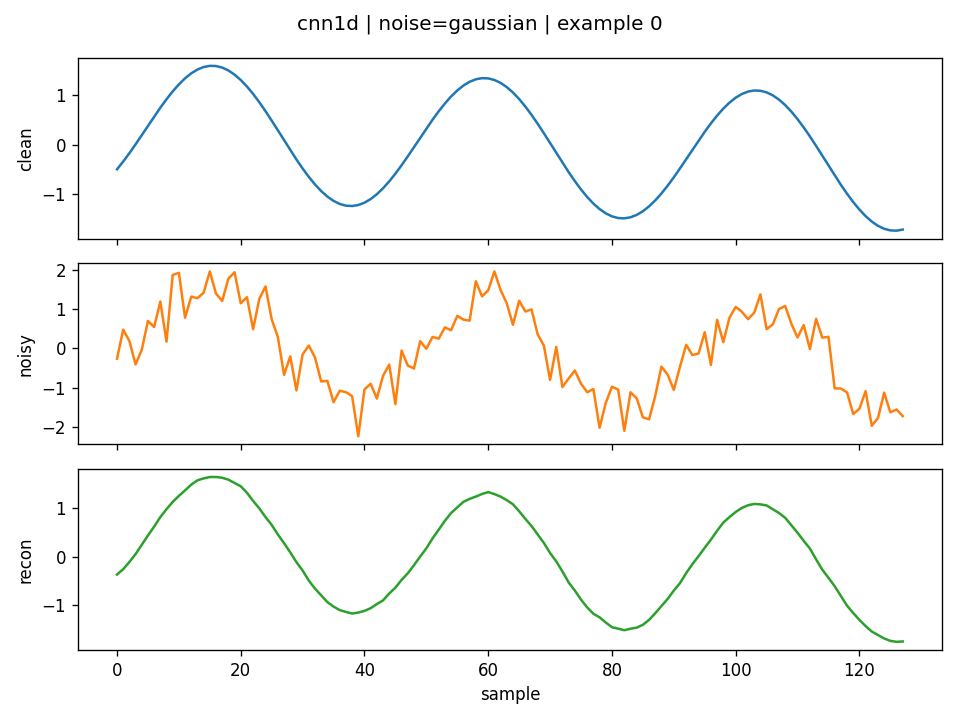
\includegraphics[width=\linewidth]{exp_3_arch/triplet_cnn1d_0.png}
\caption{CNN1D.}
\end{subfigure}
\caption{Per-architecture clean / noisy / reconstruction triplets on the same synthetic test window.}
\label{fig:triplets}
\end{figure}

\subsection{Latent dimension sweep (Exp 4)}

\begin{table}[h]
\centering
\caption{Latent-dimension sweep with the CNN architecture. The elbow falls between latent 8 and 16; gains beyond 16 are negligible.}
\label{tab:latent}
\begin{tabular}{rrrr}
\toprule
$\dim(z)$ & Params & Test MSE $\downarrow$ & $\Delta$SNR (dB) $\uparrow$ \\
\midrule
\phantom{0}4  & \phantom{0}28\,725  & 0.01407 & 11.56 \\
\phantom{0}8  & \phantom{0}36\,921  & 0.00559 & 14.91 \\
\textbf{16} & \textbf{53\,313} & \textbf{0.00527} & \textbf{15.17} \\
32 & \phantom{0}86\,097  & 0.00535 & 15.19 \\
64 & 151\,665 & 0.00534 & 15.16 \\
\bottomrule
\end{tabular}
\end{table}

The bottleneck is binding only at $z = 4$. By $z = 8$ the model has nearly saturated, and $z = 16$ achieves the best test MSE; further increases yield no improvement and triple the parameter count by $z = 64$. We adopt $z = 16$ as the default for all subsequent experiments.

\begin{figure}[h]
\centering
\begin{subfigure}{0.45\linewidth}
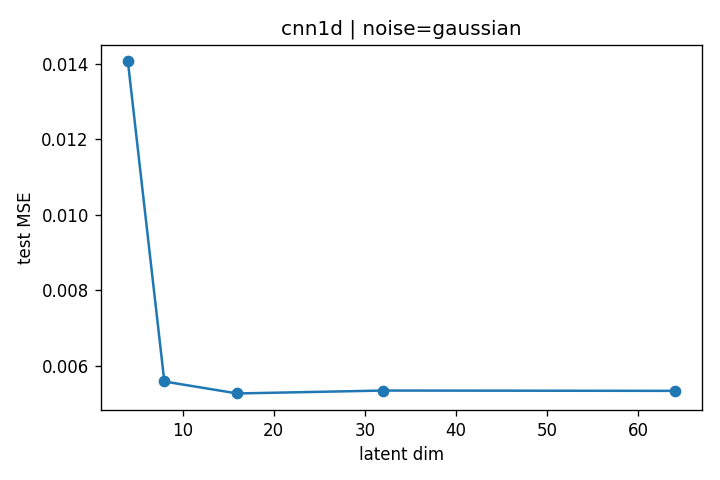
\includegraphics[width=\linewidth]{exp_4_latent/mse_vs_latent.png}
\caption{Test MSE vs.\ latent dimension.}
\end{subfigure}
\hfill
\begin{subfigure}{0.45\linewidth}
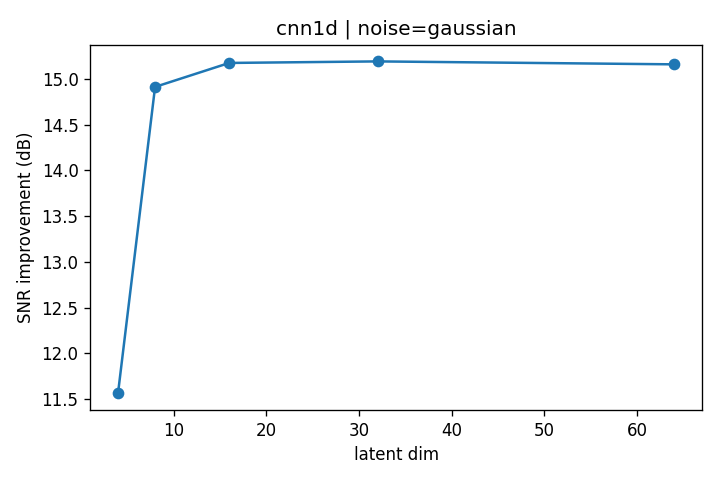
\includegraphics[width=\linewidth]{exp_4_latent/snr_imp_vs_latent.png}
\caption{SNR improvement vs.\ latent dimension.}
\end{subfigure}
\caption{Latent-dimension sweep. Performance saturates by $z = 16$.}
\label{fig:latent_sweep}
\end{figure}

\subsection{Cross-noise robustness (Exp 5)}

\begin{table}[h]
\centering
\caption{Cross-noise robustness: SNR improvement (dB) on the test set when training on row noise and evaluating on column noise. Diagonal entries are matched; off-diagonal entries are out-of-distribution.}
\label{tab:robustness}
\begin{tabular}{lrrr}
\toprule
& \multicolumn{3}{c}{Eval noise} \\
\cmidrule(lr){2-4}
Train noise & gaussian & masking & impulse \\
\midrule
gaussian & 15.13 & 11.07 & \phantom{$-$}9.74 \\
masking  & \phantom{0}6.26 & \textbf{25.17} & $-2.14$ \\
impulse  & 11.52 & \phantom{0}7.93 & \textbf{24.55} \\
\bottomrule
\end{tabular}
\end{table}

Two findings stand out. First, matched train/eval noise gives substantially higher gains (mean diagonal $= 21.6$\,dB) than mismatched (mean off-diagonal $= 7.4$\,dB). Specialization is real and sizeable. Second, the Gaussian-trained model is the most robust transfer: it never drops below 9.7\,dB on any test noise, whereas the masking-trained model actively \emph{harms} the signal on impulse noise ($-2.14$\,dB). For a single deployment-ready model, Gaussian is the safest choice --- which lines up with its also being the noise model that best fit the real residuals.

\begin{figure}[h]
\centering
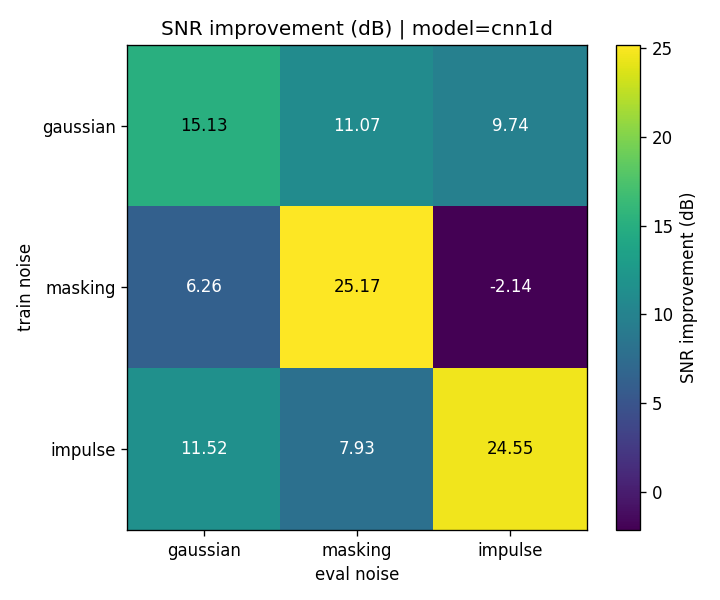
\includegraphics[width=0.65\linewidth]{exp_5_noise_robustness/robustness_heatmap.png}
\caption{Cross-noise SNR-improvement heatmap. Diagonal dominance is clear; the masking $\to$ impulse cell is the only one with negative improvement.}
\label{fig:robustness}
\end{figure}

\subsection{Noise-level generalization (Exp 6)}

\begin{table}[h]
\centering
\caption{CNN trained at the fitted Gaussian intensity ($\sigma = 0.380$, multiplier 1.0) and evaluated across a $\times 0.25$--$\times 3$ range.}
\label{tab:levels}
\begin{tabular}{rrrrr}
\toprule
Multiplier & SNR$_{\text{in}}$ (dB) & SNR$_{\text{out}}$ (dB) & $\Delta$SNR (dB) & Test MSE \\
\midrule
0.25 & 20.48 & 28.71 & \phantom{0}8.23 & 0.0016 \\
0.5  & 14.46 & 27.07 & 12.61 & 0.0024 \\
0.75 & 10.94 & 25.28 & 14.34 & 0.0037 \\
\textbf{1.0}  & \textbf{8.44} & \textbf{23.57} & \textbf{15.13} & \textbf{0.0055} \\
1.5  & \phantom{0}4.92 & 20.59 & 15.67 & 0.0110 \\
2.0  & \phantom{0}2.42 & 18.15 & 15.73 & 0.0193 \\
3.0  & $-1.10$ & 14.42 & 15.52 & 0.0452 \\
\bottomrule
\end{tabular}
\end{table}

The CNN's $\Delta$SNR plateau lies on the high-noise side of the training intensity. From multiplier $0.75$ through $3.0$ it stays within a 1.4\,dB band ($14.3$--$15.7$\,dB). Below $\sim\!0.75\times$ noise, the input is already cleaner than the model's training distribution, so the achievable improvement falls --- the model continues to denoise but the headroom is smaller. We see no catastrophic degradation in the tested range; the model gracefully extends to $3\times$ the training intensity.

\begin{figure}[h]
\centering
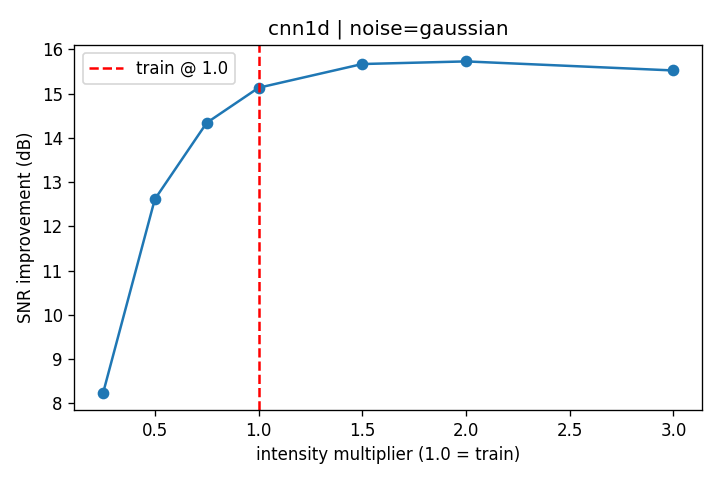
\includegraphics[width=0.7\linewidth]{exp_6_noise_levels/snr_imp_vs_intensity.png}
\caption{SNR improvement vs.\ evaluation intensity multiplier (red dashed line marks the training intensity, multiplier 1.0). The model maintains $> 14$\,dB improvement across nearly the entire tested range.}
\label{fig:levels}
\end{figure}

\subsection{Per-article sine recovery (Exp 7)}\label{sec:results-recovery}

Our first real-data evaluation applies the trained CNN to the exact task it was trained for, using the per-article fitted sines as the clean signals. For each article we take the fitted sine $\hat{y}^{(\text{art})}[t]$ as ground truth, corrupt it with Gaussian noise at the fitted intensity ($\sigma = 0.380$), run the trained CNN, and compare the reconstruction to the known sine. This is a direct per-article test of the denoiser against signals whose parameters come from the actual dataset. We average over $N = 20$ noise realizations per article. We also (a) pass the clean sine through the autoencoder unmodified to measure the baseline distortion the model itself introduces, and (b) sweep the noise intensity by the same multipliers used in Exp 6.

\begin{table}[h]
\centering
\caption{Per-article sine recovery. Each row averages over $N = 20$ noise realizations at the fitted intensity. The ``clean pass'' column is the SNR when the autoencoder is fed the clean sine itself --- a measure of the residual distortion the network introduces on top of denoising.}
\label{tab:sine_recovery}
\begin{tabular}{lrrrrr}
\toprule
Article & MSE recon $\downarrow$ & SNR$_{\text{in}}$ (dB) & SNR$_{\text{recon}}$ (dB) & $\Delta$SNR (dB) $\uparrow$ & SNR$_{\text{clean pass}}$ (dB) \\
\midrule
Influenza   & 0.0138 & 28.07 & 38.37 & 10.30 & 64.77 \\
Common\_cold & 0.0150 & 27.61 & 37.55 & \phantom{0}9.94 & 66.49 \\
Fever       & 0.0174 & 27.53 & 36.80 & \phantom{0}9.26 & 68.43 \\
Cough       & 0.0190 & 26.30 & 35.21 & \phantom{0}8.91 & 71.19 \\
\textbf{Christmas} & \textbf{0.0095} & 28.38 & \textbf{40.31} & \textbf{11.93} & 56.44 \\
\midrule
\textit{mean} & \textit{0.0149} & \textit{27.58} & \textit{37.65} & \textit{10.07} & \textit{65.46} \\
\bottomrule
\end{tabular}
\end{table}

The CNN improves SNR against the known sine by $+8.9$ to $+11.9$\,dB per article, with a mean of $+10.07$\,dB. The clean-pass SNRs (mean 65.5\,dB, range 56--71\,dB) indicate that the model leaves a clean sine essentially unchanged, so it is not adding artifacts on top of denoising. \texttt{Christmas} shows the largest improvement, consistent with its having the largest seasonal amplitude and therefore the most headroom for noise removal.

\begin{figure}[h]
\centering
\begin{subfigure}{0.49\linewidth}
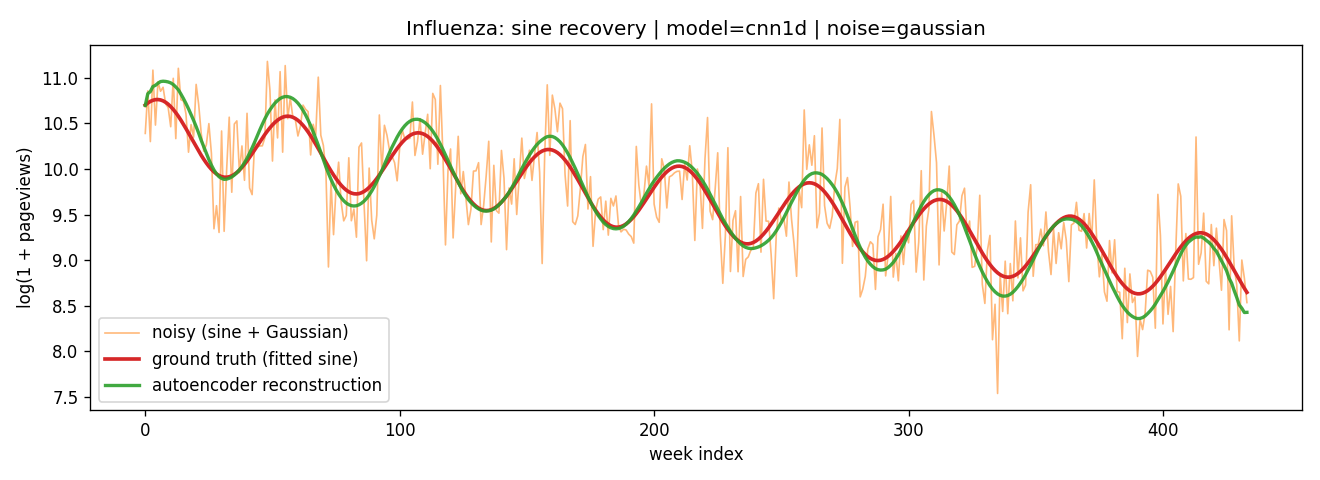
\includegraphics[width=\linewidth]{exp_8_sine_recovery/Influenza_sine_recovery.png}
\caption{Influenza.}
\end{subfigure}
\hfill
\begin{subfigure}{0.49\linewidth}
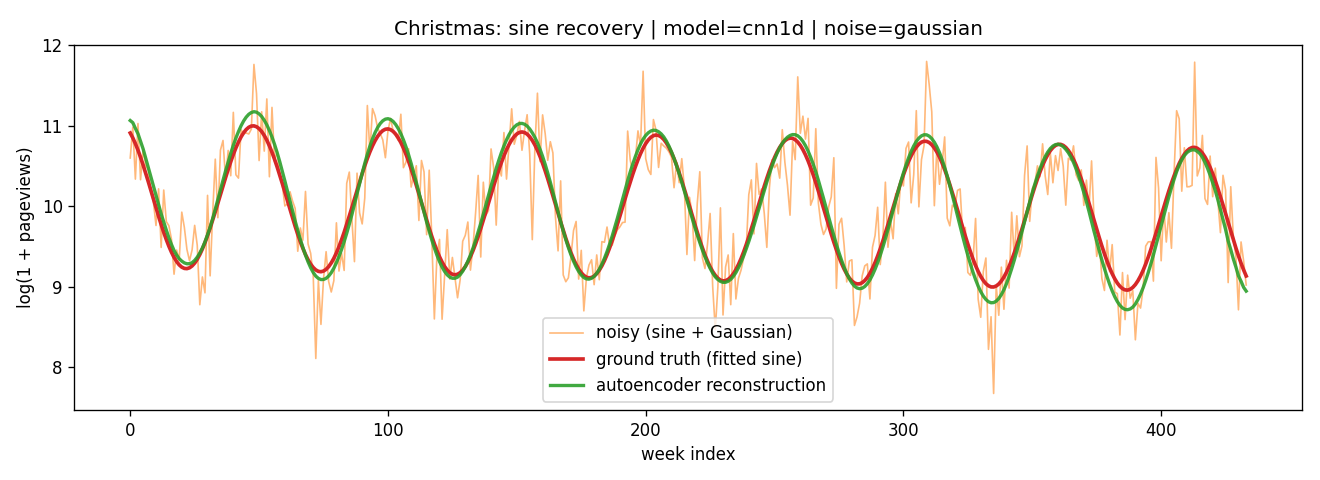
\includegraphics[width=\linewidth]{exp_8_sine_recovery/Christmas_sine_recovery.png}
\caption{Christmas.}
\end{subfigure}
\caption{Sine recovery: noisy realization (orange), known fitted sine (red, ground truth), autoencoder reconstruction (green). The reconstruction tracks the known sine closely.}
\label{fig:sine_recovery}
\end{figure}

\paragraph{Sweep across noise intensities.} Table~\ref{tab:sine_recovery_levels} and Figure~\ref{fig:sine_recovery_heatmap} report SNR improvement when the corruption noise is scaled by multipliers $\{0.25, 0.5, 0.75, 1.0, 1.5, 2.0, 3.0\}$. The pattern is consistent across articles: improvement peaks near multiplier $1.0$ (the training intensity) at 11--14\,dB, and degrades smoothly but never catastrophically away from it. At the heaviest intensity tested ($3\times$), all five articles still see $\geq 8.8$\,dB improvement.

\begin{table}[h]
\centering
\caption{Sine recovery, noise-intensity sweep ($\Delta$SNR in dB). Bold marks the trained intensity (multiplier 1.0).}
\label{tab:sine_recovery_levels}
\begin{tabular}{lrrrrrrr}
\toprule
Article & 0.25$\times$ & 0.5$\times$ & 0.75$\times$ & \textbf{1.0$\times$} & 1.5$\times$ & 2.0$\times$ & 3.0$\times$ \\
\midrule
Influenza   & 12.84 & 11.39 & 10.19 & \textbf{11.29} & \phantom{0}9.08 & \phantom{0}9.33 & 8.82 \\
Common\_cold & 12.95 & 11.03 & 10.03 & \textbf{11.49} & \phantom{0}8.75 & \phantom{0}9.03 & 8.87 \\
Fever       & 12.52 & 10.15 & \phantom{0}9.04 & \textbf{11.76} & \phantom{0}8.31 & \phantom{0}8.43 & 8.98 \\
Cough       & 11.18 & \phantom{0}8.96 & \phantom{0}8.74 & \textbf{12.93} & \phantom{0}8.23 & \phantom{0}8.17 & 9.22 \\
Christmas   & 12.88 & 12.48 & 12.36 & \textbf{14.25} & \phantom{0}9.80 & 10.38 & 9.54 \\
\bottomrule
\end{tabular}
\end{table}

\begin{figure}[h]
\centering
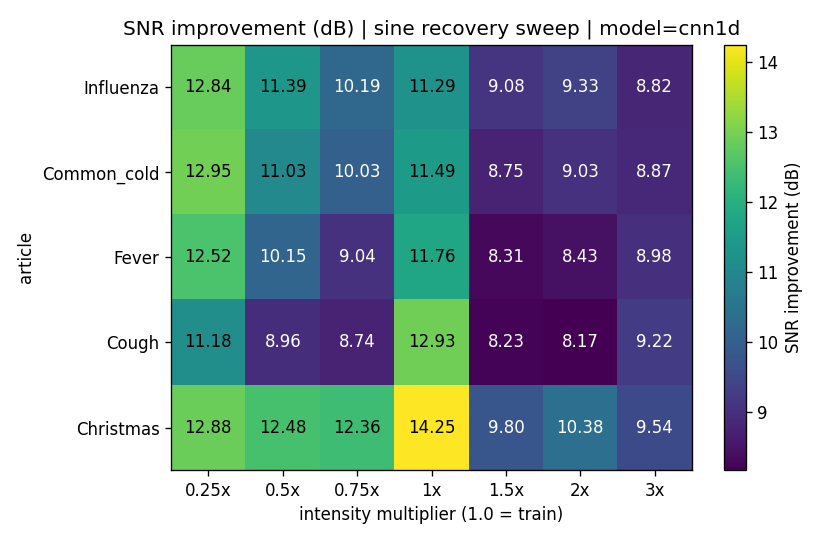
\includegraphics[width=0.85\linewidth]{exp_8_sine_recovery/sine_recovery_heatmap.png}
\caption{Sine-recovery SNR improvement (dB) per (article, intensity multiplier).}
\label{fig:sine_recovery_heatmap}
\end{figure}

\subsection{Real-data extension: windowed evaluation on raw series (Exp 8)}\label{sec:results-real}

As an extension beyond the controlled sine-recovery test, we apply the same trained CNN to the raw Wikipedia log-pageview series themselves. Unlike Exp 7, the input here is not a known clean sine plus noise but the real observed series, which contains both noise and non-stationary structure (year-to-year amplitude variation, slow phase drift). No true ground truth exists in this setting; we use the per-article fitted sine from Section~\ref{sec:results-fit} as a proxy to measure reconstruction error. Per article we slide 128-week windows with stride 1, z-score each window, run it through the autoencoder, un-z-score, and overlap-average to reconstitute a single denoised series of length $T = 472$.

\begin{table}[h]
\centering
\caption{Real-data evaluation. SNR is measured against the per-article fitted sine (Section~\ref{sec:results-fit}); $\Delta$SNR is the improvement of the autoencoder reconstruction over the raw real series.}
\label{tab:real_eval}
\begin{tabular}{lrrrr}
\toprule
Article & MSE vs.\ sine $\downarrow$ & SNR$_{\text{recon}}$ (dB) & SNR$_{\text{real}}$ (dB) & $\Delta$SNR (dB) $\uparrow$ \\
\midrule
Influenza   & 0.0855 & 30.37 & 27.74 & 2.63 \\
Common\_cold & 0.0656 & 31.06 & 28.41 & 2.65 \\
Fever       & 0.0160 & 37.12 & 32.96 & 4.16 \\
Cough       & 0.0493 & 30.99 & 28.72 & 2.27 \\
\textbf{Christmas} & 0.0502 & \textbf{32.99} & 24.94 & \textbf{8.06} \\
\bottomrule
\end{tabular}
\end{table}

The reconstruction is closer to the fitted sine than the raw real series for every article, by $+2.3$ to $+8.1$\,dB. This improvement is smaller than in Exp 7 because the input here is a real series rather than a sine-plus-noise window: the per-window reconstruction captures non-stationary variation in addition to removing noise, and counted against the single global sine, that extra detail shows up as error even though it reflects real signal structure. \texttt{Christmas} sees the largest improvement, consistent with its having the largest seasonal amplitude and the most headroom for high-frequency noise removal. \texttt{Fever} has the lowest absolute MSE (its annual amplitude is small, so per-window SNR is dominated by small absolute deviations). \texttt{Cough}, whose sine fit was degenerate (300-week period, Section~\ref{sec:results-fit}), still sees a modest improvement of 2.3\,dB.

\begin{figure}[h]
\centering
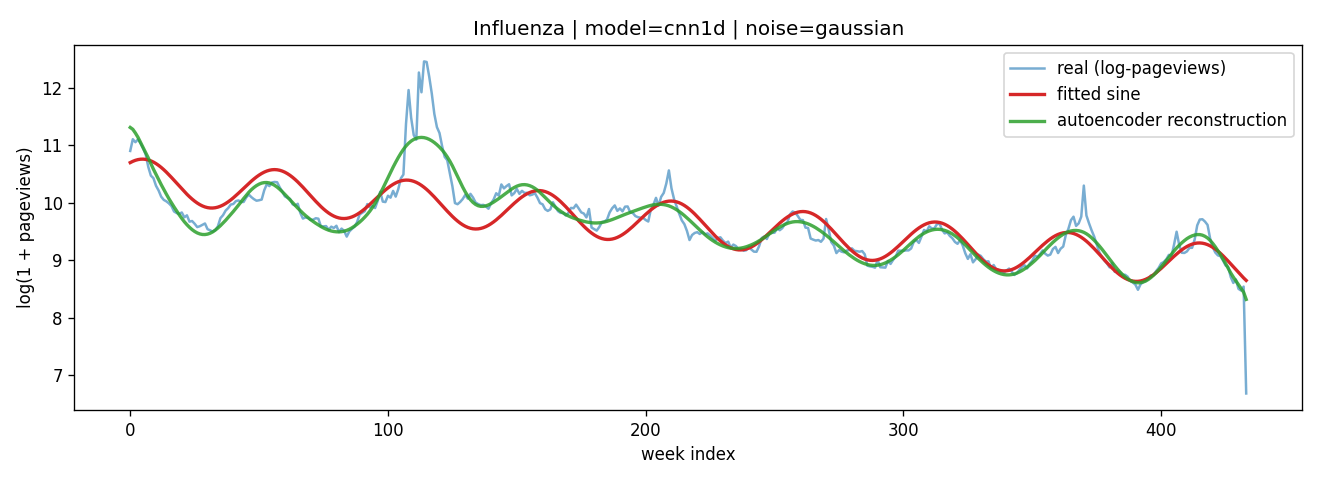
\includegraphics[width=0.95\linewidth]{exp_7_real_eval/Influenza_real_eval.png}
\caption{Influenza: real series (blue), fitted sine (red), CNN autoencoder reconstruction (green). The reconstruction follows non-stationary amplitude variation that a single global sine cannot represent --- e.g., the strong 2017--2019 seasons vs.\ the muted 2020--2021 seasons.}
\label{fig:real_eval}
\end{figure}

\section{Discussion}\label{sec:discussion}

\paragraph{Interpreting the real-data extension.}
Figure~\ref{fig:real_eval} shows the autoencoder reconstruction (green) tracking the real series more closely than the fitted sine (red). The model was trained on a \emph{distribution} of sines spanning the full range of amplitudes, frequencies, phases, slopes and offsets observed across articles --- with $\pm 50\%$ jitter on frequency in particular. At inference each 128-week window of the real series is treated independently and gets denoised toward whichever member of the trained family best matches that window. Since real Influenza amplitude varies year-to-year and phase drifts slowly, the per-window family member differs from the global fit, and the overlap-averaged reconstruction inherits this local adaptivity. The autoencoder therefore acts as a locally adaptive sine smoother on the real series rather than a regression to a single sine, which is the expected behavior given how the training distribution was constructed.

\paragraph{Comparing Exp 7 and Exp 8.}
The two real-data numbers --- $+8.9$ to $+11.9$\,dB on per-article sine recovery (Table~\ref{tab:sine_recovery}) versus $+2.3$ to $+8.1$\,dB on the raw Wikipedia series (Table~\ref{tab:real_eval}) --- differ by roughly 5--7\,dB. Exp 7 matches the model's training assumption (input = sine $+$ Gaussian noise, target = sine), and the $\sim$10\,dB improvement there quantifies pure denoising performance under matched conditions. Exp 8 measures a different quantity: how close the overlap-averaged reconstruction gets to the global fitted sine on real data, where the reconstruction is also tracking non-stationary structure (amplitude variation, phase drift) that the global sine cannot represent. Counted against the global sine, that extra structure is ``error'' even though it is real. So $\Delta$SNR vs.\ the fitted sine on real data conflates two effects: (a) pure noise removal, which Exp 7 isolates and quantifies at $\sim$10\,dB, and (b) richer modeling of slow non-stationary structure, which subtracts a few dB from (a) when the metric is taken against the deliberately limited sine target. A stricter proxy (a low-pass filter at the annual frequency, a top-$k$ Fourier reconstruction, or an STL decomposition) would isolate (a) on the raw-series extension the way Exp 7 does by construction.

\paragraph{Heavy-tailed residuals and Gaussian noise.}
Section~\ref{sec:results-noise} flagged that the fitted Gaussian under-models the residual kurtosis. In principle a heavier-tailed noise model (e.g., Student-$t$ or a Gaussian--impulse mixture) might be a better real-data fit, but our spec restricts us to the three project-prescribed families. Within those, Gaussian wins on bulk distribution and is also the most robust transfer (Table~\ref{tab:robustness}); the trade-off between bulk fit and tail fit appears unavoidable with the available choices.

\paragraph{Cough degeneracy.}
\texttt{Cough}'s fit lands on a 300-week period instead of $\sim 52$ weeks (Table~\ref{tab:sine_fits}). The article's annual cycle has lower amplitude than its long-term trend and seasonal sub-modes, so the FFT-initialized fit collapses to a long-period mode. We made no attempt to debias the fit (e.g., by detrending more aggressively, or restricting the frequency search to the annual band) because we wanted a uniform pipeline across articles. The downstream autoencoder still produces a reasonable denoising for \texttt{Cough} --- it operates on local windows and is not restricted to the global sine --- but the reported real-data SNR for \texttt{Cough} is the noisiest of the five.

\paragraph{Limitations.}
(i) The synthetic clean signal family is narrow (single dominant sinusoid plus linear trend); richer composite signals (multiple frequencies, sparse spike events) would be a logical extension. (ii) The real-data evaluation is anchored to a deliberately limited proxy; a richer baseline would tighten the interpretation. (iii) Five Wikipedia articles is a small sample; expanding to a broader article set would test how well the parameter ranges generalize.

\section{Conclusion}

This project implemented an end-to-end denoising-autoencoder pipeline whose synthetic benchmark is grounded in a real time-series dataset. The pipeline (i) extracts a dominant-sinusoid model from real Wikipedia pageview series, (ii) characterizes the residual distribution and selects the best-fitting noise model from a fixed candidate set, (iii) generates synthetic training data from the fitted sine distribution corrupted by the selected noise model, (iv) trains and compares two autoencoder architectures, (v) evaluates the trained CNN on a per-article sine-recovery task that matches the training assumptions, and (vi) applies the same model as an extension to the raw real Wikipedia series via overlap-averaged sliding windows. The 1D CNN provides the best trade-off among the tested architectures: $+15.2$\,dB SNR improvement on synthetic data with roughly half the parameter count of the MLP, a clean latent-dimension knee at 16, and robust generalization to noise intensities up to $3\times$ training. On the per-article sine-recovery task it achieves $+10.1$\,dB mean improvement with near-identity behavior on clean sines ($\sim$65\,dB). As an extension to the raw Wikipedia series, the same model yields $+2.3$ to $+8.1$\,dB improvement against the fitted-sine proxy; the reduced gain reflects that the per-window reconstruction also captures non-stationary structure (amplitude variation, phase drift) that the global sine cannot represent.

\paragraph{Code availability.}
All code, configs, and exact reproduction instructions are in the project repository, under \texttt{src/}, \texttt{experiments/}, and \texttt{configs/}. A single command \texttt{python experiments/run\_all.py} reproduces every table and figure in this report. A pytest suite under \texttt{tests/} exercises the data, model, and evaluation layers.

\begin{thebibliography}{9}
\bibitem{wikimedia}
Wikimedia Foundation. \emph{Wikimedia REST API: Pageviews.}\\
\url{https://wikimedia.org/api/rest_v1/}
\bibitem{generous}
N.~Generous, G.~Fairchild, A.~Deshpande, S.~Y.~Del Valle, R.~Priedhorsky.
``Global disease monitoring and forecasting with Wikipedia.''
\emph{PLOS Computational Biology}, 10(11):e1003892, 2014.
\bibitem{vincent}
P.~Vincent, H.~Larochelle, Y.~Bengio, P.-A.~Manzagol.
``Extracting and composing robust features with denoising autoencoders.''
\emph{ICML}, 2008.
\end{thebibliography}

\end{document}
